\documentclass[10pt,twocolumn]{article}
\usepackage[letterpaper,top=0.75in,bottom=1in,left=0.625in,right=0.625in,columnsep=0.25in]{geometry}
\usepackage{times}\usepackage{mathptmx}
\usepackage[T1]{fontenc}\usepackage[utf8]{inputenc}
\usepackage{amsmath,amssymb,graphicx,booktabs,array,cite,url,microtype,caption,titlesec,float}
\usepackage[hidelinks]{hyperref}
\captionsetup{font=footnotesize,labelfont=footnotesize,labelsep=period,skip=3pt}
\captionsetup[table]{labelfont=footnotesize,textfont=sc,labelformat=simple,labelsep=newline,justification=centering}
\renewcommand{\thetable}{\Roman{table}}
\titleformat{\section}{\centering\normalfont\footnotesize\scshape}{\thesection.}{0.5em}{}
\titleformat{\subsection}{\normalfont\footnotesize\itshape}{\thesubsection)}{0.5em}{}
\renewcommand{\thesection}{\Roman{section}}
\renewcommand{\thesubsection}{\Alph{subsection}}
\titlespacing*{\section}{0pt}{8pt}{4pt}\titlespacing*{\subsection}{0pt}{5pt}{2pt}
\setlength{\parindent}{10pt}\setlength{\parskip}{0pt}
\renewcommand{\arraystretch}{1.08}
\setlength{\textfloatsep}{8pt plus 2pt minus 2pt}\setlength{\floatsep}{6pt plus 2pt minus 2pt}\setlength{\intextsep}{6pt plus 2pt minus 2pt}
\pagestyle{plain}
\begin{document}
\twocolumn[
\begin{center}
{\LARGE\bfseries Building and Pre-training a Character-Level GPT from Scratch:\\[2pt] Architecture, Compute-Constrained Optimisation and an Analysis of the Evaluation Protocol\par}
\vspace{8pt}
{\large Manidip Debnath\par}
{\small\itshape Oakland University, Rochester, Michigan, USA\par}
{\small manidipdeb@oakland.edu\par}
\vspace{10pt}
\end{center}
\begin{center}\begin{minipage}{0.93\textwidth}
\small\noindent\textbf{\textit{Abstract}---}This report documents the complete work of a course assignment: implementing a nanoGPT-style decoder-only transformer from scratch (tokenizer, batching, causal attention, MLP, block, full model, learning-rate schedule, training step, text generation), pre-training it on 40\,M characters of TinyStories, and then minimising its validation loss under a fixed budget of $2\times10^{14}$ FLOPs. The 0.82\,M-parameter default model reaches 0.8585 nats/char (perplexity 2.36, 1.24 bits/char), below the required 1.00. A two-stage search (12\%-budget screening, six full-budget runs, fresh-seed replication) selects a context of 256 characters with batch size 8, which reaches \textbf{0.7016} nats/char (1.012 bits/char, perplexity 2.02) against 0.7478 for the baseline, below the 0.725 top tier on all three seeds. Follow-up experiments then show that this gain is entirely an effect of how the specified evaluation averages over windows of the model's own length: scored with equal windows, the longer-context model is not better. They also show that the chosen model size is close to the best at this budget, that dropout hurts, and that rotary position embeddings (RoPE), which win at 35\% of the budget (0.8476 against 0.8555), lose at the full budget (0.7212 against 0.7060). All six written questions of the assignment are answered in full with derivations and evidence from the experiments.
\end{minipage}\end{center}
\begin{center}\begin{minipage}{0.93\textwidth}\small\noindent\textbf{\textit{Index Terms}---}language model, transformer, GPT, TinyStories, character-level tokenization, compute-constrained training, scaling, rotary position embedding, evaluation protocol.\end{minipage}\end{center}
\vspace{6pt}]

\section{Introduction}
Generative pre-trained transformers (GPT) learn to predict the next token of a text and, with scale, acquire fluent language ability \cite{radford2019,vaswani2017}. Training a large model is out of reach for a course project, but the \emph{recipe} is the same at small scale: a data pipeline, a tokenizer, a causal transformer, an optimiser with a learning-rate schedule, and a careful evaluation. TinyStories \cite{eldan2023} makes the small scale meaningful: children's-story text with a limited vocabulary lets models below one million parameters write mostly grammatical English.

This report follows the structure of the assignment, which is based on nanoGPT \cite{karpathy2022}. Its contributions are:
\begin{enumerate}
\item a from-scratch implementation of every component of the pipeline, with the ten required unit tests (Sections~\ref{sec:data}--\ref{sec:gen});
\item a default model that meets the validation-loss requirement ($\le1.00$ nats/char) and a compute-budgeted search that reaches 0.7016 nats/char, together with a fresh-seed replication (Section~\ref{sec:res});
\item an analysis of the evaluation protocol showing that the whole gain from a longer context is a scoring effect (Section~\ref{sec:window}), a study of model size, dropout and batch size (Section~\ref{sec:size}), and a rotary-embedding extension that does not survive the full budget (Section~\ref{sec:rope});
\item complete answers to the six written questions (Section~\ref{sec:qa}) and a mapping of the work to the grading rubric (Appendix~\ref{app:rubric}).
\end{enumerate}

\section{Background}
\subsection{Language modelling objective}
A language model assigns a probability to a token sequence $x_1,\dots,x_n$. By the chain rule,
\begin{equation}
p(x_1,\dots,x_n)=\prod_{t=1}^{n}p(x_t\mid x_1,\dots,x_{t-1}),
\end{equation}
so it suffices to model the next-token distribution. The model is trained by minimising the cross-entropy
\begin{equation}
\mathcal{L}(\theta)=-\frac1N\sum_{t=1}^{N}\log p_\theta(x_{t+1}\mid x_{1:t}),
\end{equation}
in nats per token. No labels are needed: the text is its own supervision, which is why this is called self-supervised pre-training.

\subsection{Reading a loss value}
Three equivalent units are used throughout. The \emph{perplexity} $e^{\mathcal L}$ is the size of a uniform distribution that would be equally uncertain. The \emph{bits per character} $\mathcal L/\ln2$ is the average code length of an ideal compressor built on the model; plain ASCII uses 8 bits, so the \emph{compression ratio} is $8/(\mathcal L/\ln2)$. An untrained model with a uniform guess over $|V|=96$ characters has $\mathcal L=\ln96=4.564$ (perplexity 96, 6.585 bits), which is the sanity check used to debug the training code.

\subsection{Scaling and compute budgets}
Training cost is approximately $6ND$ FLOPs for $N$ parameters and $D$ tokens, plus an attention term that grows with the context length \cite{kaplan2020}. For a fixed budget there is a trade-off between model size and number of tokens; the compute-optimal point is at roughly 20 tokens per parameter \cite{hoffmann2022}. The assignment asks to find a good point in this trade-off on a small scale, which is the subject of Section~\ref{sec:size}.

\section{Data and Tokenization}\label{sec:data}
\subsection{Corpus}
The training text is the first 40\,MB of the TinyStories V2 training file (48,793 stories, 39,963,595 characters after cleaning); the validation text is the official validation file (27,629 stories, 22,482,104 characters). Stories are separated by the end-of-text marker \texttt{<|endoftext|>}. Curly quotes and dashes are mapped to ASCII, and only newline plus the 95 printable ASCII characters are kept. The model never trains on the validation text.

\begin{figure}[t]\centering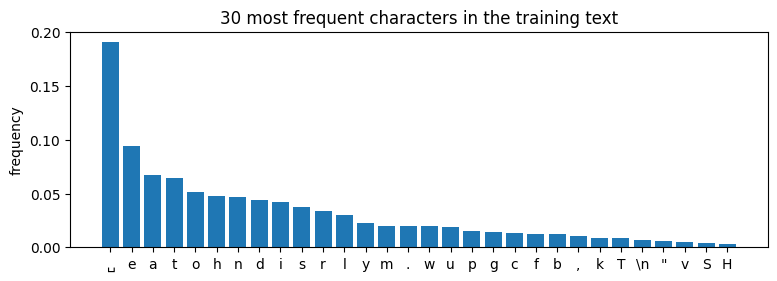
\includegraphics[width=\columnwidth]{figures/cell018.png}
\caption{Thirty most frequent characters of the training text; the space alone is about 19\% of the text.}\label{fig:freq}\end{figure}

\subsection{TODO 1: character-level tokenizer}
The vocabulary has $|V|=96$ entries and token id $i$ is character \texttt{VOCAB[i]}. Two dictionaries are built with comprehensions, \texttt{stoi = \{ch: i for i, ch in enumerate(VOCAB)\}} and its inverse \texttt{itos}; \texttt{encode} maps a string to a list of ids and \texttt{decode} joins characters back. The test checks \texttt{encode("Hi!") == [41, 74, 2]} and exact round trips. A character-level vocabulary makes the output layer tiny (12\,K parameters at $d=128$, against 6.4\,M for a 50,257-token BPE vocabulary) at the price of longer sequences (Q5).

\subsection{TODO 2: next-token batches}
A batch is built by drawing \texttt{batch\_size} random start positions $i$ and stacking the windows \texttt{data[i:i+T]} (inputs) and \texttt{data[i+1:i+T+1]} (targets), i.e.\ the targets are the inputs shifted left by one. One window of length $T$ therefore gives $T$ training examples at once. The test verifies shapes $(B,T)$, dtype \texttt{int64}, the shift property, and that every row equals the expected slice.

\section{Model Architecture}\label{sec:model}
The model (Fig.~\ref{fig:arch}) is a pre-norm decoder-only transformer. Token embeddings \texttt{wte} and learned position embeddings \texttt{wpe} are added, passed through $n_{\text{layer}}=4$ blocks, a final LayerNorm and a linear head that is tied to \texttt{wte}.

\begin{figure}[t]\centering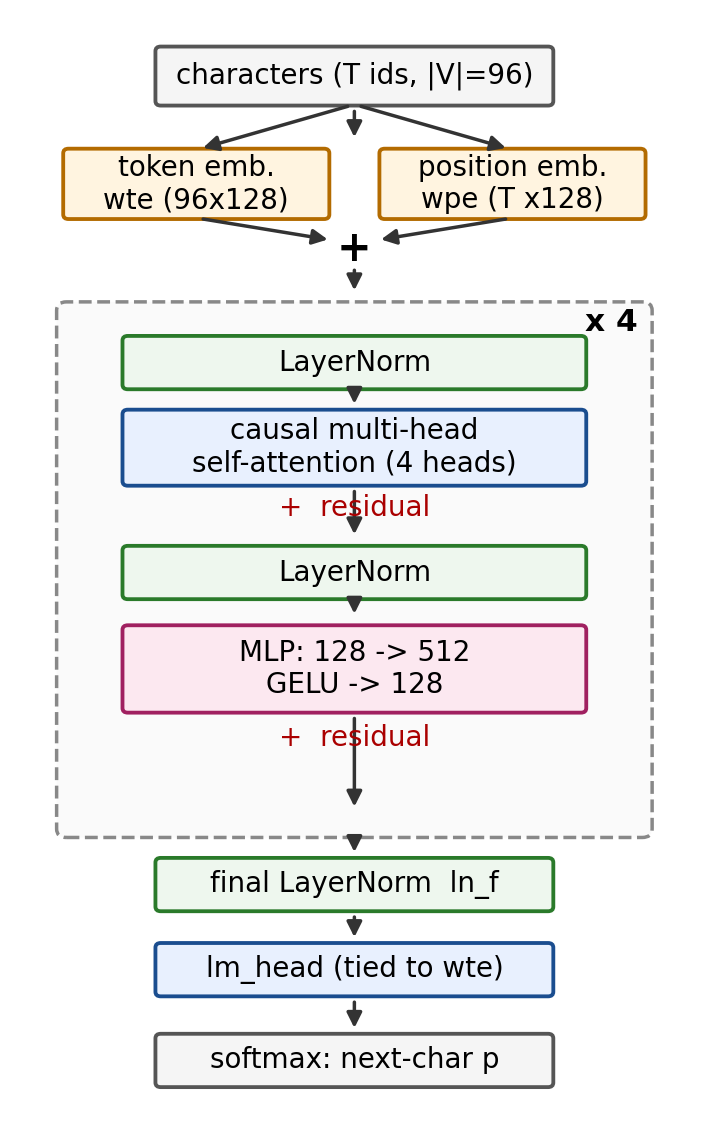
\includegraphics[width=0.62\columnwidth]{figures/fig_architecture.png}
\caption{Architecture of the implemented GPT (default: $d=128$, 4 heads, 4 blocks).}\label{fig:arch}\end{figure}

\subsection{TODO 3: causal scaled dot-product attention}
For $Q,K,V\in\mathbb{R}^{T\times d_k}$ and a mask $M$ with $M_{ij}=0$ for $j\le i$ and $-\infty$ otherwise,
\begin{equation}
\mathrm{Attn}(Q,K,V)=\mathrm{softmax}\!\Big(\tfrac{QK^{\top}}{\sqrt{d_k}}+M\Big)V.
\end{equation}
The implementation computes the scores \texttt{q @ k.transpose(-2,-1) / sqrt(d\_k)}, fills the future positions with $-\infty$ using \texttt{masked\_fill(\textasciitilde mask, -inf)}, applies \texttt{softmax} over the last dimension and multiplies with $V$. The test compares the result with PyTorch's \texttt{scaled\_dot\_product\_attention(is\_causal=True)} and checks that the first token sees only itself.

\subsection{TODO 4: multi-head attention}
One fused linear layer \texttt{c\_attn} (width $3d$) produces $Q,K,V$ for all heads; each is reshaped $(B,T,d)\to(B,T,h,d_k)\to(B,h,T,d_k)$ with \texttt{view} and \texttt{transpose}, passed through \texttt{causal\_attention}, merged back and projected by $W_O$ (\texttt{c\_proj}). With $h=4$ heads of width $d_k=32$ every head can learn a different ``who looks at whom'' pattern. The test changes only the last tokens and verifies that earlier outputs do not change (causality), and compares against a reference built from PyTorch's attention.

\subsection{TODO 5 and 6: MLP and transformer block}
The MLP is $\mathrm{MLP}(x)=W_2\,\mathrm{GELU}(W_1x+b_1)+b_2$ with $W_1\in\mathbb{R}^{4d\times d}$ \cite{hendrycks2016}; it processes every position independently and holds about two thirds of the parameters. A block uses residual connections and pre-LayerNorm \cite{ba2016}:
\begin{equation}
x\leftarrow x+\mathrm{Attn}(\mathrm{LN}_1(x)),\quad x\leftarrow x+\mathrm{MLP}(\mathrm{LN}_2(x)).
\end{equation}
Residual paths let gradients flow unchanged through deep stacks; normalising before each sub-layer keeps activations at a stable scale.

\subsection{TODO 7: the full model and its loss}
The forward pass looks up \texttt{tok\_emb = wte(idx)} and \texttt{pos\_emb = wpe(arange(T))}, adds them (broadcasting over the batch), runs the blocks, applies \texttt{ln\_f} and \texttt{lm\_head}, and, if targets are given, flattens logits to $(BT,|V|)$ and targets to $(BT)$ for \texttt{F.cross\_entropy}. Two provided details matter: weight tying (\texttt{lm\_head.weight = wte.weight}) saves parameters, and GPT-2 initialisation draws weights from $\mathcal N(0,0.02^2)$ and uses the smaller std $0.02/\sqrt{2n_{\text{layer}}}$ for projections that write into the residual stream. The test checks the initial loss against $\ln96$, that the loss is a scalar, that future tokens do not change earlier logits, and that gradients reach \texttt{wpe} and every block.

\subsection{Parameter count}
The estimate $12d^2$ per block gives $4\cdot12\cdot128^2=786{,}432$ plus embeddings $96\cdot128+128\cdot128=28{,}672$, i.e.\ 815,104. The model has \textbf{822,016} parameters; the difference of 6,912 is exactly the biases and LayerNorm parameters ($1{,}664$ per block $\times4$ plus 256 for \texttt{ln\_f}). The tied head adds nothing. A context of 256 adds 128 rows to the position table (+16,384), giving 838,400.

\section{Training Procedure}\label{sec:train}
\subsection{Optimiser and schedule (TODO 8)}
We use AdamW ($\beta=(0.9,0.99)$) \cite{loshchilov2019} with weight decay 0.1 on matrices and embeddings only (not on biases and LayerNorm) and gradient clipping at norm 1.0. The learning rate follows a linear warm-up and cosine decay,
\begin{equation}
\eta(s)=\begin{cases}\eta_{\max}\frac{s+1}{s_w}, & s<s_w,\\[2pt] \eta_{\min}+\tfrac12(\eta_{\max}-\eta_{\min})(1+\cos\pi r), & \text{else},\end{cases}
\end{equation}
with $r=(s-s_w)/(s_{\max}-s_w)$, $\eta_{\max}=3\times10^{-3}$, $\eta_{\min}=3\times10^{-4}$ and $s_w=100$ (200 in the long runs). Warm-up avoids large noisy steps while the weights are random; decay makes late steps smaller and finer. The test checks $\eta(0)=\eta_{\max}/100$, $\eta(49)=\eta_{\max}/2$, the peak after warm-up, the midpoint of the decay and the end value.

\subsection{One training step (TODO 9)}
A step is four lines: forward pass \texttt{logits, loss = model(xb, yb)}; \texttt{optimizer.zero\_grad(set\_to\_none=True)}; \texttt{loss.backward()}; \texttt{optimizer.step()}. Gradients must be cleared at every step because PyTorch accumulates them. A 200-step smoke test must bring the loss below 2.5.

\subsection{Compute accounting}
Training compute is estimated as \cite{kaplan2020}
\begin{equation}
C\approx\big(6N+12\,n_{\text{layer}}\,d\,T\big)\times D,\quad D=\text{steps}\times B\times T.
\end{equation}
The attention term grows with $T$, so at a fixed $C$ a longer context sees fewer tokens. A budget planner converts a fraction of $C_{\max}=2\times10^{14}$ into a number of steps with exactly this formula, so no run can exceed the budget; the full-budget runs use 99.5\%.

\section{Text Generation (TODO 10)}\label{sec:gen}
Generation feeds the last \texttt{block\_size} tokens, takes the logits at the last position, divides them by a temperature $\tau$, applies softmax and samples one token with \texttt{torch.multinomial}:
\begin{equation}
p_i=\frac{e^{z_i/\tau}}{\sum_je^{z_j/\tau}}.
\end{equation}
Low $\tau$ sharpens the distribution (safer, more repetitive; $\tau\to0$ is greedy decoding), high $\tau$ flattens it. Top-$k$ sampling \cite{fan2018} keeps only the $k$ largest logits. The test checks the output shape, that the prompt is preserved, that prompts longer than \texttt{block\_size} are cropped, and that \texttt{top\_k=1} and a tiny temperature both reproduce greedy decoding.

\section{Evaluation Protocol}\label{sec:eval}
\subsection{Fixed-slice loss}
The training-time \texttt{estimate\_loss} averages random batches and is noisy (standard error about 0.003--0.004). All comparisons therefore use the deterministic \emph{fixed-slice} loss of the assignment's Part~8: the first $10^6$ validation characters are cut into consecutive windows of the model's own \texttt{block\_size} and the mean cross-entropy over all windows is reported. Because the window length equals the model's context length, this choice matters, as Section~\ref{sec:window} shows.

\subsection{Reference baselines}
Table~\ref{tab:base} gives context-free references from training counts and the default and final models.

\begin{table}[t]\centering\caption{Baselines and models on the fixed validation slice}\label{tab:base}
\footnotesize\begin{tabular}{lcccc}\toprule
Model & Loss & Perplexity & bits/char & Compr.\\\midrule
Uniform & 4.5643 & 96.00 & 6.585 & 1.2$\times$\\
Unigram & 3.0806 & 21.77 & 4.444 & 1.8$\times$\\
Bigram & 2.2800 & 9.78 & 3.289 & 2.4$\times$\\
Default GPT (3,000 steps) & 0.8585 & 2.36 & 1.239 & 6.5$\times$\\
\textbf{Final GPT (full budget)} & \textbf{0.7016} & \textbf{2.02} & \textbf{1.012} & \textbf{7.9}$\times$\\\bottomrule\end{tabular}\end{table}

\section{Experimental Results}\label{sec:res}
\subsection{Default model (Part 5)}
The default model (3,000 steps, batch 32, $T=128$, 822,016 parameters) uses $7.03\times10^{13}$ FLOPs (35\% of the budget) and trains in 0.8 minutes on a Tesla T4. Training and validation loss fall together from $\ln96\approx4.56$ (Fig.~\ref{fig:default}), pass 2.5 within the first 250 steps and end at 0.8687 (train) and 0.8495 (validation, \texttt{estimate\_loss}). On the deterministic slice the loss is \textbf{0.8585} nats/char, perplexity 2.36, 1.239 bits/char and 6.5$\times$ compression, which meets the requirement of at most 1.00 with a wide margin (10 of 10 points). There is no overfitting: training and validation loss are equal within noise.

\begin{figure}[t]\centering
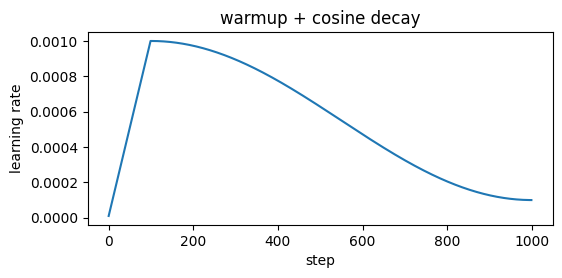
\includegraphics[width=0.49\columnwidth]{figures/cell049.png}\hfill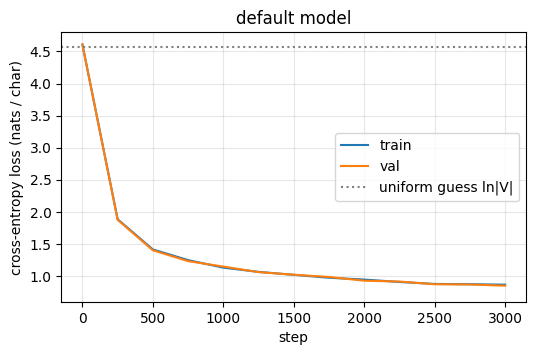
\includegraphics[width=0.49\columnwidth]{figures/cell057.png}
\caption{Left: warm-up and cosine-decay schedule (unit-test plot, $\eta_{\max}=10^{-3}$, 1,000 steps). Right: training and validation loss of the default model; the dotted line is $\ln|V|$.}\label{fig:default}\end{figure}

\subsection{Search protocol (Part 7)}
The score of Part~7 depends on the Part~8 loss of one model trained with \texttt{train()} within $C_{\max}$ (tiers: $\le0.85$ 8 points, $\le0.80$ 12, $\le0.76$ 16, $\le0.74$ 18, $\le0.725$ 20). Fig.~\ref{fig:flow} summarises the protocol. The rule for choosing the final model was fixed before the runs: take the setting with the lowest fixed-slice loss at the full budget (seed 1337), then replicate the winner and the baseline with two fresh seeds, because selecting on one seed favours the winner. Only the knobs context length, batch size, learning rate and weight decay are changed in the search, and every run uses at most $0.995\,C_{\max}$.

\begin{figure*}[t]\centering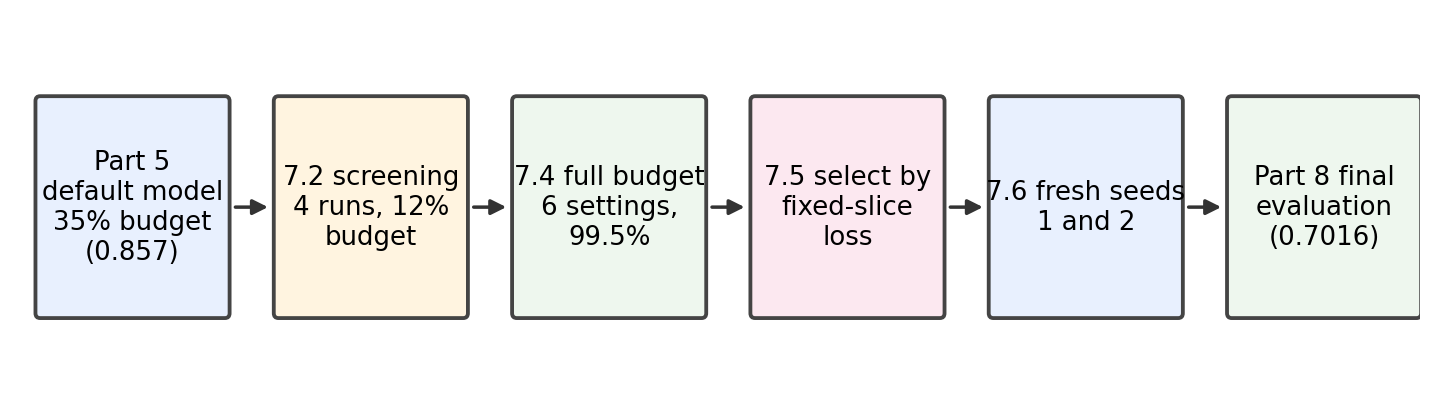
\includegraphics[width=0.85\textwidth]{figures/fig_workflow.png}\caption{Experimental workflow of Part~7.}\label{fig:flow}\end{figure*}

\subsection{Screening at 12\% of the budget}
Four candidates were trained for 12\% of the budget (Table~\ref{tab:screen}, Fig.~\ref{fig:screen}). A candidate had to beat the baseline by a margin of 0.010, chosen in advance; none did (best: weight decay 0.01, $-0.0070$), so screening alone would have kept the baseline. The context-256 candidate ranked \emph{last} (+0.1772).

\begin{table}[t]\centering\caption{Screening runs (12\% budget, fixed-slice loss)}\label{tab:screen}
\footnotesize\begin{tabular}{lcc}\toprule
Candidate & Loss & vs.\ base\\\midrule
wd 0.01 & 1.0979 & $-0.0070$\\
base ($\eta=3\mathrm{e}{-3}$) & 1.1050 & 0\\
$\eta=2\mathrm{e}{-3}$ & 1.1527 & $+0.0478$\\
context 256 (batch 16) & 1.2821 & $+0.1772$\\\bottomrule\end{tabular}\end{table}

\begin{figure}[t]\centering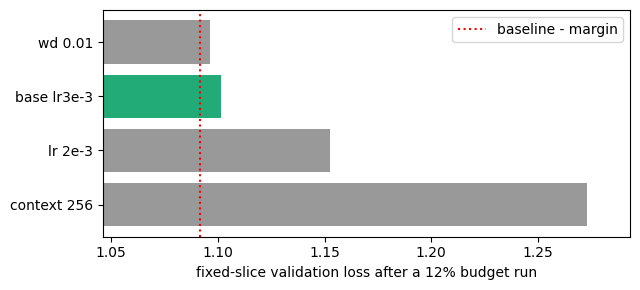
\includegraphics[width=0.92\columnwidth]{figures/cell079.png}\caption{Screening result. The red line is the baseline minus the 0.010 margin.}\label{fig:screen}\end{figure}

\subsection{Full-budget runs}
Because short runs can mislead, six settings were then trained with 99.5\% of the budget (2.3--2.9 minutes each on a T4). Table~\ref{tab:full} gives the result and Fig.~\ref{fig:curves} the learning curves; Fig.~\ref{fig:compute} shows every run against its compute.

\begin{table}[t]\centering\caption{Full-budget runs (seed 1337, fixed-slice loss)}\label{tab:full}
\footnotesize\begin{tabular}{lrrcr}\toprule
Setting & Params & Steps & Loss & $\Delta$\\\midrule
\textbf{T256, batch 8} & 838,400 & 14,715 & \textbf{0.7016} & $-0.0462$\\
T256, batch 16, $\eta{=}4\mathrm{e}{-3}$ & 838,400 & 7,357 & 0.7067 & $-0.0411$\\
T384, batch 8 & 854,784 & 8,650 & 0.7211 & $-0.0267$\\
T512, batch 8 & 871,168 & 5,802 & 0.7251 & $-0.0227$\\
T256, batch 16 & 838,400 & 7,357 & 0.7343 & $-0.0135$\\
T128, batch 32 (baseline) & 822,016 & 8,495 & 0.7478 & 0\\\bottomrule\end{tabular}\end{table}

\begin{figure*}[t]\centering
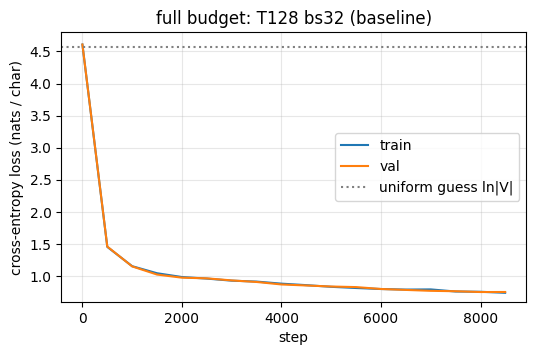
\includegraphics[width=0.32\textwidth]{figures/cell082.png}\hfill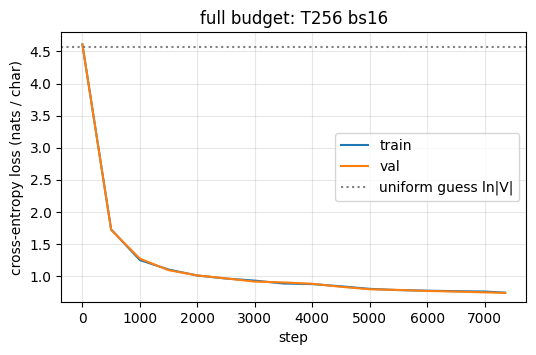
\includegraphics[width=0.32\textwidth]{figures/cell083.png}\hfill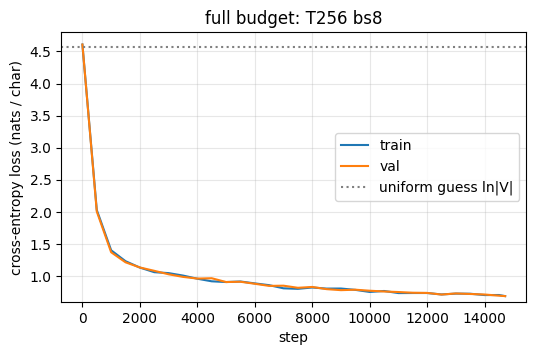
\includegraphics[width=0.32\textwidth]{figures/cell084.png}\\[3pt]
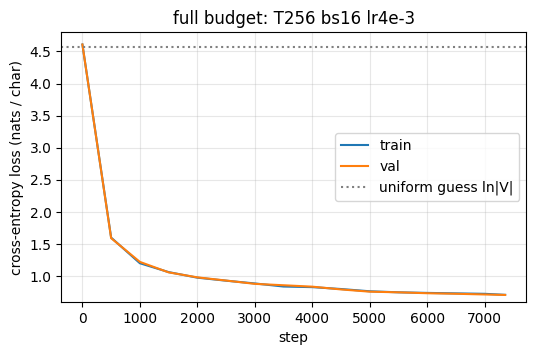
\includegraphics[width=0.32\textwidth]{figures/cell085.png}\hfill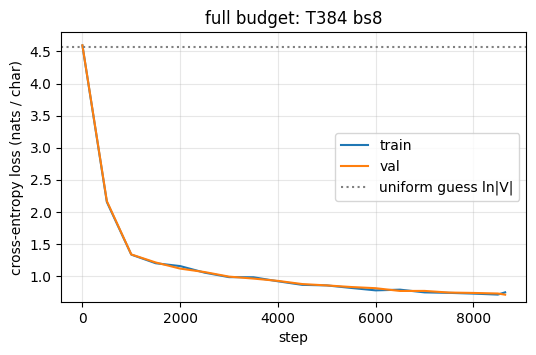
\includegraphics[width=0.32\textwidth]{figures/cell086.png}\hfill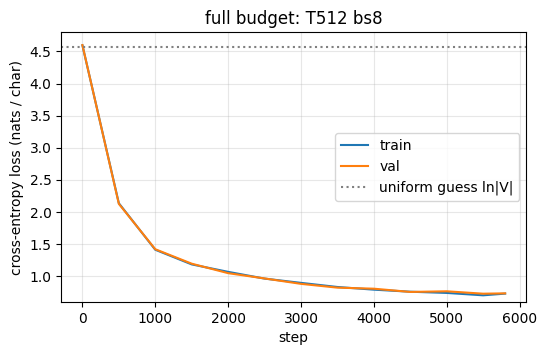
\includegraphics[width=0.32\textwidth]{figures/cell087.png}
\caption{Training and validation loss of the six full-budget runs (top: T128 bs32 baseline, T256 bs16, T256 bs8; bottom: T256 bs16 $\eta{=}4\mathrm{e}{-3}$, T384 bs8, T512 bs8).}\label{fig:curves}\end{figure*}

\begin{figure*}[t]\centering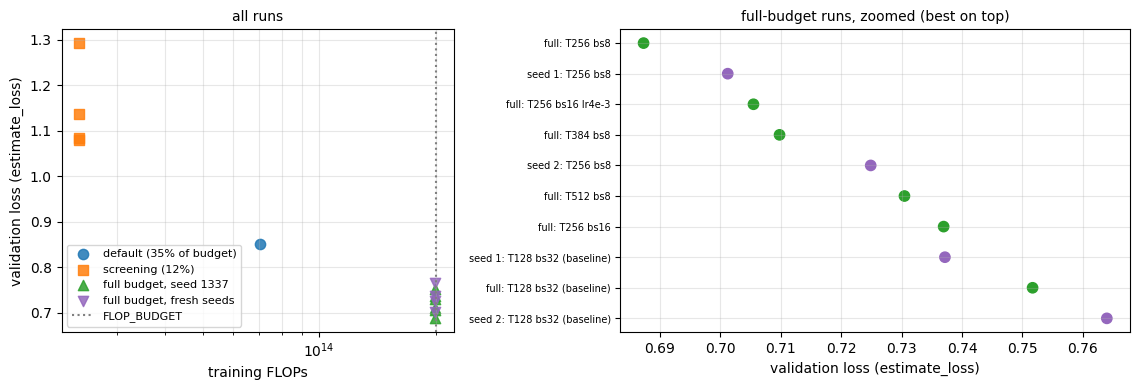
\includegraphics[width=0.9\textwidth]{figures/cell099.png}\caption{Validation loss (from \texttt{estimate\_loss}) against training FLOPs for every run. Left: all runs; right: the full-budget runs ranked, best on top (green: seed 1337, purple: fresh seeds).}\label{fig:compute}\end{figure*}

Moving from context 128 to 256 at equal tokens per step (batch 16) lowers the Part~8 loss by 0.0135; halving the batch to 8 doubles the updates and lowers it by a further 0.0327, and a higher learning rate at batch 16 gets most of the same gain (0.7067). Contexts longer than 256 did not pay off: the attention term makes every token more expensive, so only 8,650 (T384) and 5,802 (T512) steps fit. A short run ranked the winning context length last, so short-run rankings did not transfer to the full budget.

\subsection{Fresh seeds}
Table~\ref{tab:seed} replicates the baseline and the winner with seeds 1 and 2. On the two fresh seeds the baseline averages 0.7544 and the winner 0.7082, a gain of 0.0461, about 12 times the larger seed standard deviation (0.0039). All three winner seeds are below the 0.725 threshold (worst 0.7088, margin 0.016), so the tier does not depend on the seed. The winner was chosen among six settings on the slice it is scored on, which favours it slightly; this is why fresh seeds are reported. The baseline itself is not exactly reproducible across sessions (0.7478, 0.7513 and 0.7552 for the same seed), so one baseline number carries about $\pm0.004$ of uncertainty, whereas the winner reproduced 0.7016 every time.

\begin{table}[t]\centering\caption{Seed replication (fixed-slice loss)}\label{tab:seed}
\footnotesize\begin{tabular}{lccccc}\toprule
Setting & 1337 & 1 & 2 & Mean & Std\\\midrule
T128 bs32 & 0.7478 & 0.7535 & 0.7553 & 0.7522 & 0.0039\\
T256 bs8 & 0.7016 & 0.7077 & 0.7088 & 0.7060 & 0.0038\\\bottomrule\end{tabular}\end{table}

\subsection{Loss by position}
Fig.~\ref{fig:pos} plots the loss against the position inside the window. At position 0 the model has seen one character and its loss (about 2.3) is close to the bigram baseline (2.28); after about ten characters it is near 1.0 and it keeps falling slowly. The longer-context model lies below the default one at almost every position. Because Part~8 averages over whole windows of the model's own length, a longer window contains a smaller share of the expensive first characters, which lowers the measured loss by itself.

\begin{figure}[t]\centering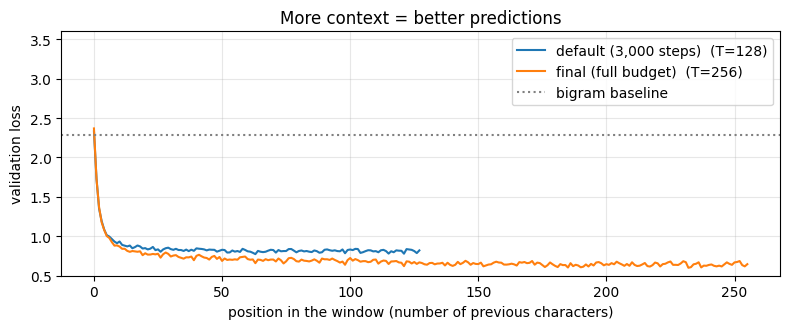
\includegraphics[width=\columnwidth]{figures/cell108.png}\caption{Fixed-slice loss by position in the window for the default (T=128) and final (T=256) models.}\label{fig:pos}\end{figure}

\subsection{Follow-up runs: the scoring effect}\label{sec:window}
The follow-up runs (Appendix~B of the notebook) use seed 1337, 99.5\% of $C_{\max}$, \texttt{train()}, and learning rate $3\times10^{-3}$ without re-tuning, in the same session as the rest of the notebook. To separate the model from the scoring, the \emph{same trained models} are scored with windows of 32, 64, 128 and 256 characters (Table~\ref{tab:win}); a model with context $T$ can be scored with any window $\le T$. With equal 128-character windows the winner (0.7532) is \emph{not} better than the baseline (0.7478). The Part~8 difference of 0.0462 splits exactly into $-0.0516$ from the window length alone (112\% of the gain) and $+0.0054$ from the model, which is within the run-to-run variation of the baseline. On windows of 32 and 64 characters the winner is worse, as expected for a model trained only on 256-character windows. The longer context therefore does not make the model a better predictor at a given context length; it lowers the metric, which averages over whole windows. This is allowed by the specified evaluation, and the final score uses it, but it must not be read as a 0.05 improvement of the language model. An evaluation with overlapping windows would remove the effect (not run).

\begin{table}[t]\centering\caption{Loss of the same models scored with different window lengths}\label{tab:win}
\footnotesize\begin{tabular}{lcccc}\toprule
Model (block size) & 32 & 64 & 128 & 256\\\midrule
T128 bs32 baseline (128) & 0.9033 & 0.8077 & 0.7478 & --\\
T128 bs8 (128) & 0.9221 & 0.8270 & 0.7700 & --\\
T256 bs8 winner (256) & 0.9274 & 0.8246 & 0.7532 & 0.7016\\\bottomrule\end{tabular}\end{table}

\subsection{Model size, batch size and dropout}\label{sec:size}
Table~\ref{tab:size} and Fig.~\ref{fig:size} change the size around the winner at the same compute. The loss is U-shaped: a smaller model that sees more text (width 96, 102 characters per parameter) is worse by 0.0275, a deeper one (6 layers, 16.5) by 0.0113 and a wider one (width 192, 8) by 0.1126. At about 36 characters per parameter, above the roughly 20 of the compute-optimal rule \cite{hoffmann2022}, the winner is close to the best trade-off among the sizes tried, so neither a bigger model nor more tokens paid off. The learning rate was not re-tuned per size, so the width-192 result may partly be a learning-rate effect. Context 128 with batch 8 (33,983 steps) gives 0.7700, worse than batch 32 (0.7478), so a smaller batch does not help by itself; the benefit seen at context 256 is therefore not a general rule. Dropout 0.1 gives 0.7826, worse by 0.0810, consistent with the absence of overfitting (the final run reads 0.75 of one pass over the data, and train and validation loss are 0.688 and 0.687). For the same reason the amount of training data (\texttt{TRAIN\_MB}) was not changed.

\begin{table}[t]\centering\caption{Same budget, different sizes (context 256, batch 8)}\label{tab:size}
\footnotesize\begin{tabular}{lrrrc}\toprule
Setting & Params & Tokens (M) & Tok./param & Loss\\\midrule
width 96 & 481,344 & 48.9 & 102 & 0.7292\\
\textbf{width 128 (winner)} & 838,400 & 30.1 & 36 & \textbf{0.7016}\\
6 layers & 1,234,944 & 20.4 & 16.5 & 0.7129\\
width 192 & 1,847,424 & 14.8 & 8 & 0.8142\\
dropout 0.1 & 838,400 & 30.1 & 36 & 0.7826\\
T128, batch 8 & 822,016 & 34.8 & 42 & 0.7700\\\bottomrule\end{tabular}\end{table}

\begin{figure}[t]\centering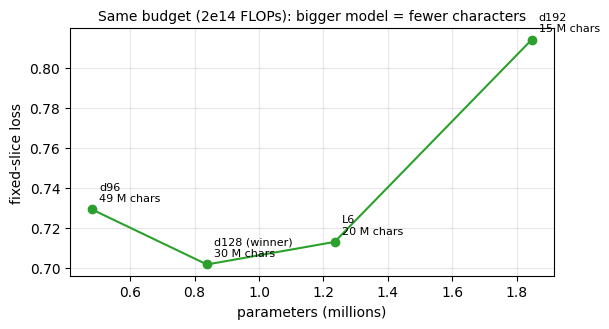
\includegraphics[width=0.92\columnwidth]{figures/fig_size.png}\caption{Loss against model size at the same compute; the labels give the number of training characters.}\label{fig:size}\end{figure}

\subsection{Sample quality}
At $\tau=0.8$, 99.1\% of the 845 words generated by the final model and 98.7\% of the 855 words of the default model occur at least three times in the training text; the difference is not significant (one standard error of a rate near 99\% is 0.4--0.5 points) and the metric cannot measure coherence. The qualitative differences across temperatures are analysed in Q4.

\section{Bonus: Rotary Position Embeddings}\label{sec:rope}
Rotary embeddings (RoPE) \cite{su2021} remove the learned position table. Each head's query and key are rotated, pair by pair, by an angle proportional to the position, $\theta_m=10000^{-2m/d_k}$, so that $\langle R_iq,R_jk\rangle$ depends only on $i-j$; the value vector is left unchanged. The RoPE model has 805,632 parameters (16,384 fewer, exactly the removed table). Four tests pass: position 0 is not rotated, rotations preserve vector length, scores are unchanged when both positions shift by the same amount, and attention remains causal (changing future tokens leaves earlier logits unchanged); an untrained RoPE model starts at $\ln96$.

\emph{At the default setting} (35\% of the budget, same configuration, learning rate, seed and data), RoPE reaches 0.8442 against 0.8585 for learned positions (paired difference $0.0143\pm0.0005$ over 7,812 windows, RoPE better on 61.9\%); its validation loss is lower at every logged step, most strongly early (1.41 against 1.85 at step 250; Fig.~\ref{fig:rope}). \emph{Three seeds} (Table~\ref{tab:rope}, Fig.~\ref{fig:ropeseeds}) give $0.8476\pm0.0032$ for RoPE against $0.8555\pm0.0026$; the gap of 0.0079 is 3.3 standard errors of the seed spread, every RoPE seed is below every learned seed (probability 1/20 if exchangeable) and a Welch test gives $p=0.031$.

\begin{figure*}[t]\centering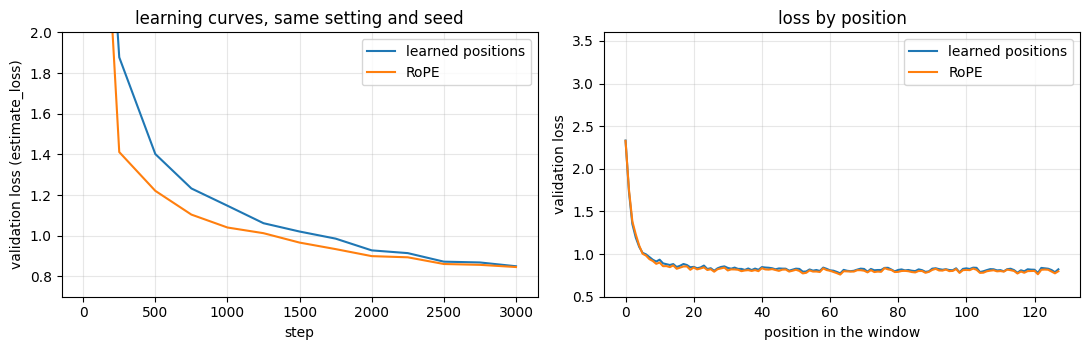
\includegraphics[width=0.9\textwidth]{figures/cell125.png}\caption{RoPE against learned positions at the default setting. Left: learning curves; right: loss by position.}\label{fig:rope}\end{figure*}

\begin{table}[t]\centering\caption{RoPE against learned positions (35\% budget)}\label{tab:rope}
\footnotesize\begin{tabular}{lccccc}\toprule
Model & 1337 & 1 & 2 & Mean & Std\\\midrule
Learned & 0.8585 & 0.8544 & 0.8536 & 0.8555 & 0.0026\\
RoPE & 0.8442 & 0.8480 & 0.8506 & 0.8476 & 0.0032\\\bottomrule\end{tabular}\end{table}

\begin{figure}[t]\centering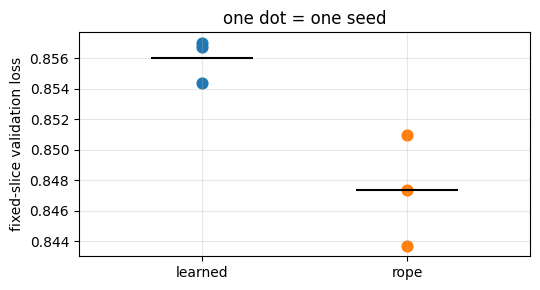
\includegraphics[width=0.8\columnwidth]{figures/cell135.png}\caption{One dot per seed; black bars are means.}\label{fig:ropeseeds}\end{figure}

\emph{At the full budget} the advantage reverses. With the winner setting (context 256, batch 8, the same 14,715 steps, three seeds) RoPE scores $0.7212\pm0.0050$ (0.7260, 0.7217, 0.7160) against $0.7060\pm0.0038$ for learned positions (0.7016, 0.7077, 0.7088); every learned seed is below every RoPE seed and Welch gives $p=0.016$. The 35\% result is therefore best read as ``RoPE learns faster early''. The learning rate was not re-tuned for RoPE and the reason was not investigated. The RoPE model is not the Part~8 model, since the final model must come from \texttt{train()}, which builds the original GPT.

\section{Answers to the Written Questions}\label{sec:qa}
\subsection*{Q1 (2 points): initial loss}
\textbf{(a)} An untrained model spreads probability evenly, so the correct token gets $1/|V|$ and the loss is $\ln|V|$. For GPT-2's $|V|=50{,}257$ this is $\ln50257\approx10.83$ nats ($\approx15.6$ bits), against $\ln96\approx4.56$ for our model: the larger the vocabulary, the more a model must learn before it beats a blind guess. \textbf{(b)} A loss of 25 means the correct token has probability about $e^{-25}\approx1.4\times10^{-11}$, far worse than the uniform guess $1/96\approx0.0104$. The model is not merely ignorant but \emph{confidently wrong}: its logits are huge and put almost all probability on wrong tokens. This points to a bug or bad initialisation (weights of too large a scale, a missing $\sqrt{d_k}$ scaling, or misaligned inputs and targets); a healthy network starts with small logits and a loss near $\ln|V|$.

\subsection*{Q2 (3 points): causal mask and $\sqrt{d_k}$}
\textbf{(a)} Without the mask, position $t$ can attend to position $t+1$, whose token is exactly the target of position $t$. The model learns to \emph{copy the answer from the input} instead of predicting it, so the training loss falls quickly towards 0 and a validation loss computed with the same unmasked attention would also look excellent but be meaningless. At generation time the next token does not exist yet, so there is nothing to copy; the model never learned to predict from the past alone and its samples are essentially garbage. \textbf{(b)} If the entries of $q$ and $k$ are independent with mean 0 and variance 1, each product $q_jk_j$ has mean 0 and variance 1, so $\mathrm{Var}(q\cdot k)=\sum_{j=1}^{d_k}\mathrm{Var}(q_jk_j)=d_k$ and a score has standard deviation $\sqrt{d_k}$, which grows with the head size. Large scores make the softmax nearly one-hot; it saturates and its gradient is close to 0, so training stalls. Dividing by $\sqrt{d_k}$ restores unit variance whatever $d_k$ is.

\subsection*{Q3 (2 points): parameter count}
Blocks: $4\times12d^2=4\times12\times128^2=786{,}432$. Embeddings: \texttt{wte} $96\times128=12{,}288$ and \texttt{wpe} $128\times128=16{,}384$, together 28,672 (the tied head adds nothing). The estimate is $786{,}432+28{,}672=815{,}104$; the model prints \textbf{822,016}. The difference of 6,912 is what the estimate ignores, the biases and LayerNorm parameters: per block the biases of \texttt{c\_attn} (384), attention \texttt{c\_proj} (128), \texttt{c\_fc} (512) and MLP \texttt{c\_proj} (128) give 1,152, and two LayerNorms with $\gamma,\beta$ give $2\cdot2\cdot128=512$, so 1,664 per block, 6,656 for four blocks, plus 256 for the final LayerNorm: $6{,}656+256=6{,}912$.

\subsection*{Q4 (2 points): temperature}
The three samples of the prompt ``One day, a little dog'' come from the same model; only $\tau$ in $p_i=e^{z_i/\tau}/\sum_je^{z_j/\tau}$ changes. \textbf{$\tau=0.5$:} dividing logits by a small number \emph{stretches} the gaps, so softmax puts most probability on the likeliest character. This is the cleanest sample: all words are real, there are quotation marks and questions, and the sentences are short and mostly grammatical (``Max was very happy and said, `Why are you sad?'\,''), although the meaning drifts (``a big street'', ``The picture was so happy''). The price is diversity: ``happy'' appears four times in a few sentences and ``a big'' returns. \textbf{$\tau=1.0$:} we sample from the learned distribution; names and sentence shapes are plausible, but non-words (``airor'', ``Miama'', ``loused'', ``twing'') and grammar breaks (``He also laughed and happy to read his friends to help'') appear, and the sample ends with the start of the end-of-text marker, showing that the model learned where stories end. \textbf{$\tau=1.5$:} dividing by a number above 1 \emph{flattens} the distribution, so unlikely characters get real probability: non-words are everywhere (``broes'', ``realing'', ``olderful'', ``brighed'', ``Ectefully''), capitals land inside words (``dtJimb''), punctuation lands in odd places (``together: shouthed'') and a story is cut after one sentence. Because every character is sampled given the previous ones, one bad character pushes the context away from the training data, the next prediction gets worse and errors compound. As $\tau\to0$ the output becomes greedy; as $\tau\to\infty$ it approaches uniform noise over the 96 characters.

\subsection*{Q5 (3 points): tokenization}
\textbf{(a)} \emph{Advantage:} the vocabulary is tiny (96 entries), so the embedding table and output layer are small (about 12\,K parameters instead of 6.4\,M at $d=128$), there are no out-of-vocabulary tokens, no tokenizer has to be trained and typos or rare names are no problem. \emph{Disadvantage:} the same text needs about 4--5 times as many tokens than with BPE \cite{sennrich2016}, so attention costs more for the same amount of text, a window of 128 tokens covers only a few sentences, and the model has to learn spelling and word boundaries before grammar. \textbf{(b)} The two losses average over different units, nats per character and nats per token, and a token carries more information than a character. The total information is the same: $L_{\text{char}}N_{\text{chars}}=L_{\text{tok}}N_{\text{tokens}}$, hence
\begin{equation}
L_{\text{char}}=L_{\text{tok}}\cdot\frac{N_{\text{tokens}}}{N_{\text{chars}}}=\frac{L_{\text{tok}}}{\text{characters per token}}.
\end{equation}
For English BPE the average is about 4 characters per token, so 3.0 nats per token is about 0.75 nats per character. Dividing by $\ln2$ gives bits per character, or bits per byte, the unit used to compare models with different tokenizers.

\subsection*{Q6 (3 points): base model versus assistant}
The model does not answer, it \textbf{continues the text}. After ``The capital of France is'' it writes a made-up word and then a story (``cluddy. Mia was sad and thanked the dog with the mountain.''), not a country or a city. After the prompt ``Question: What is the capital of France? Answer:'' it continues with story-like text (``I can make that it is a tall!'' Ben smiled and said\ldots'') and never names a city. The only objective it ever saw was next-character prediction on TinyStories, which contains neither facts about France nor any question-and-answer format, so nothing rewards an answer; even a much larger web-trained base model would continue the text rather than reliably answer. Turning a base model into a chat assistant needs further stages: (1) \emph{supervised fine-tuning} on many instruction--response examples, which teaches the format ``a question gets an answer''; (2) \emph{preference tuning}, where humans or AI rank several responses and the model is optimised towards the preferred ones, with RLHF (a reward model and PPO) \cite{ouyang2022,schulman2017} or a direct method such as DPO \cite{rafailov2023}; (3) often safety data and, more recently, reinforcement learning on tasks with verifiable answers. Knowledge itself comes from pre-training on a much larger and broader corpus.

\subsection*{Experiment discussion (5 points)}
\textbf{What helped most.} (i) \emph{Compute}: the default model (0.8585) improves to 0.7478 with the full budget, a drop of 0.1107. (ii) \emph{Longer context with a smaller batch}: the winner scores 0.7016 (mean of three seeds $0.7060\pm0.0038$) against $0.7522\pm0.0039$ for the baseline, about 12 times the seed noise, but Section~\ref{sec:window} shows that this gain is entirely a window-length effect of the Part~8 score. \textbf{What did not help:} the learning rate 2e-3 (+0.0478 in screening), the context of 256 in the 12\% screening (ranked last, yet best at the full budget), contexts of 384 and 512 (fewer steps), dropout (+0.0810), a smaller batch at context 128, and RoPE at the full budget. \textbf{Overfitting:} none; train and validation loss are 0.688 and 0.687 in the final run, which reads 0.75 of one pass. \textbf{Bigger model or more tokens?} Neither: width 96 (more tokens) is worse by 0.0275, 6 layers by 0.0113 and width 192 (fewer tokens) by 0.1126, so the winner at about 36 characters per parameter is near the optimum of the sizes tried (Table~\ref{tab:size}).

\section{Discussion and Threats to Validity}
\textbf{Compute mattered most.} Using the full budget instead of 35\% lowers the baseline from 0.8585 to 0.7478, much more than any architectural change. \textbf{Short-run rankings are unreliable}: the winning context length ranked last at 12\%. \textbf{The metric shapes the winner.} The Part~8 score averages over windows of the model's own length, so a longer context is rewarded even when the model is no better at a fixed context length; the selection was legitimate under the rules, but the improvement should be reported as a property of the protocol, as done here. \textbf{Limitations:} one hardware type (a T4; GPU runs are not bit-for-bit reproducible and the baseline varied by about $\pm0.004$ across sessions); selection on a single slice (mitigated by fresh seeds); one seed for each follow-up run; no learning-rate re-tuning for other sizes or for RoPE; three seeds for the RoPE comparisons; no evaluation with overlapping windows.

\section{Conclusion}
A from-scratch character-level GPT with 0.82\,M parameters reaches 0.8585 nats/char with the default setting and \textbf{0.7016} nats/char (perplexity 2.02, 1.01 bits/char, 7.9$\times$ compression) under a $2\times10^{14}$-FLOP budget, with context 256 and batch 8, on all three seeds below the top-tier threshold of 0.725. The gain over the baseline is 12 times the seed noise, but all of it is explained by scoring longer windows, not by a better model. Around the winner, a smaller or larger model, more or fewer tokens, dropout and a different batch size are all worse. Rotary embeddings help at 35\% of the budget (0.8476 against 0.8555) but not at the full budget (0.7212 against 0.7060). Future work: overlapping-window evaluation, per-size learning-rate tuning, more seeds, and RoPE at the full budget with its own tuning.

\appendix
\renewcommand{\thesection}{\Alph{section}}
\section{Implementation checklist}\label{app:impl}
\begin{table}[H]\centering\caption{Assignment components and their tests}\label{tab:todo}
\footnotesize\begin{tabular}{llc}\toprule
Part & Component & Points\\\midrule
TODO 1 & \texttt{stoi}, \texttt{itos}, \texttt{encode}, \texttt{decode} & 4\\
TODO 2 & \texttt{get\_batch} & 5\\
TODO 3 & \texttt{causal\_attention} & 6\\
TODO 4 & \texttt{CausalSelfAttention.forward} & 5\\
TODO 5 & \texttt{MLP.forward} & 3\\
TODO 6 & \texttt{Block.forward} & 4\\
TODO 7 & \texttt{GPT.forward} & 8\\
TODO 8 & \texttt{get\_lr} & 5\\
TODO 9 & one training step in \texttt{train()} & 5\\
TODO 10 & \texttt{generate} & 5\\\bottomrule\end{tabular}\end{table}
All ten test cells print their check mark in the saved run, and all locked (\texttt{Do not modify}) cells are unchanged from the course notebook.

\section{Mapping to the grading rubric}\label{app:rubric}
\begin{table}[H]\centering\caption{Rubric and estimated score}\label{tab:rubric}
\footnotesize\begin{tabular}{p{1.55in}ccp{0.85in}}\toprule
Item & Max & Est. & Evidence\\\midrule
TODOs 1--10 & 50 & 50 & all tests pass\\
Default model $\le1.00$ & 10 & 10 & 0.8585\\
Part 7 model & 20 & 20 & 0.7016, 1.99e14 FLOPs\\
Log and discussion & 5 & 5 & 11 runs, answers above\\
Q1--Q6 & 15 & 14--15 & Section~\ref{sec:qa}\\
Bonus (RoPE) & +10 & +9--10 & Section~\ref{sec:rope}\\\bottomrule\end{tabular}\end{table}

\section*{Acknowledgment}
This report accompanies the notebook \texttt{nanogpt\_pretraining\_final\_Manidip\_Debnath\_v5.ipynb}; all numbers are taken from its executed outputs (one run on a Google Colab Tesla T4).

\begin{thebibliography}{99}\footnotesize
\bibitem{vaswani2017}A.~Vaswani \emph{et al.}, ``Attention is all you need,'' in \emph{Proc.\ NeurIPS}, 2017.
\bibitem{radford2019}A.~Radford \emph{et al.}, ``Language models are unsupervised multitask learners,'' OpenAI, 2019.
\bibitem{karpathy2022}A.~Karpathy, ``nanoGPT,'' 2022. [Online]. Available: \url{https://github.com/karpathy/nanoGPT}
\bibitem{eldan2023}R.~Eldan and Y.~Li, ``TinyStories: How small can language models be and still speak coherent English?'' arXiv:2305.07759, 2023.
\bibitem{kaplan2020}J.~Kaplan \emph{et al.}, ``Scaling laws for neural language models,'' arXiv:2001.08361, 2020.
\bibitem{hoffmann2022}J.~Hoffmann \emph{et al.}, ``Training compute-optimal large language models,'' arXiv:2203.15556, 2022.
\bibitem{su2021}J.~Su \emph{et al.}, ``RoFormer: Enhanced transformer with rotary position embedding,'' arXiv:2104.09864, 2021.
\bibitem{loshchilov2019}I.~Loshchilov and F.~Hutter, ``Decoupled weight decay regularization,'' in \emph{Proc.\ ICLR}, 2019.
\bibitem{ba2016}J.~L.~Ba, J.~R.~Kiros and G.~E.~Hinton, ``Layer normalization,'' arXiv:1607.06450, 2016.
\bibitem{hendrycks2016}D.~Hendrycks and K.~Gimpel, ``Gaussian error linear units (GELUs),'' arXiv:1606.08415, 2016.
\bibitem{fan2018}A.~Fan, M.~Lewis and Y.~Dauphin, ``Hierarchical neural story generation,'' in \emph{Proc.\ ACL}, 2018.
\bibitem{sennrich2016}R.~Sennrich, B.~Haddow and A.~Birch, ``Neural machine translation of rare words with subword units,'' in \emph{Proc.\ ACL}, 2016.
\bibitem{ouyang2022}L.~Ouyang \emph{et al.}, ``Training language models to follow instructions with human feedback,'' in \emph{Proc.\ NeurIPS}, 2022.
\bibitem{schulman2017}J.~Schulman \emph{et al.}, ``Proximal policy optimization algorithms,'' arXiv:1707.06347, 2017.
\bibitem{rafailov2023}R.~Rafailov \emph{et al.}, ``Direct preference optimization: Your language model is secretly a reward model,'' in \emph{Proc.\ NeurIPS}, 2023.
\end{thebibliography}
\end{document}
